\chapter{Introduction}

Page-based virtual memory transparently allocates different parts of the physical memory to each process in units of fixed-sized pages. The translations between virtual and physical addresses are stored in a hierarchy of page tables (4 levels in modern AMD64 systems). The Translation Lookaside Buffer (TLB) caches virtual-to-physical translations so that the memory-management unit (MMU) does not need to walk the page tables for every memory access. The TLB is critical to performance and TLB misses add significant overhead to execution time in many workloads \cite{Barr}. Superpages offer a significant reduction in TLB misses by allowing larger regions of memory to be represented with one TLB entry. AMD64 supports creating 2MB and 1GB superpages by setting a flag in the page table entries that stops the page table walk before the last level. The TLB has separate groups of entries for 2MB, 1GB, and the regular 4KB pages.

The Linux kernel has a system called Transparent Hugepages (THP) which automatically creates 2MB superpages whenever large blocks of memory are allocated or previously-allocated blocks of memory are found to be alligned to 2MB \cite{THP}. This enables any program to gain the advantages of superpages without being written with them in mind. To maintain transparency to userspace, THP are automatically split whenever an operation is done that would change a page's properties, such as write-protecting memory.

While superpages can increase TLB reach and thus reduce misses, they are less flexible than 4KB pages because they map a larger contiguous region of memory. The main example this paper investigates is copy-on-write, where two processes map a region of their virtual address space to the same page until one of them writes to the page. At that point, the page is copied, the writing process changes its mapping to the new page, and only the new page receives the write. This allows processes to share as much memory as possible, reducing memory usage and increasing performance. With superpages, much of this benefit is lost because even a small write forces the entire large region to be copied. Alternatively, a transparent hugepage could be split when a copy-on-write occurs to allow only 4KB to be copied, but this gives up the TLB miss savings. Transparent hugepages are not currently split by default for COW.

Our solution to this problem is to use a system called overlays to allow more flexible management of superpages and achieve the best of both worlds. In addition to the existing mapping from a virtual superpage to contiguous physical memory, each 4KB page with the superpage can optionally map to an overlay, which overrides the virtual-to-physical mapping for that page. The set of pages within a superpage that map to overlays is defined by the overlay bit vector (OBitVector). With this system, copy-on-write can be replaced with overlay-on-write. Instead of copying the entire superpage, an overlay is created for one 4KB region in the address space of the writing process. Thus, only 4KB needs to be copied and the rest of the superpage still exists for both processes, providing the usual memory utilization and TLB reach improvements.

The superpage overlay system presented here is based on page overlays from another recent work \cite{Seshadri}. That framework used overlays the size of a cache line for very fine-grained management of regular pages. Superpage overlays are simpler in that they can simply extend the existing page table system and thus require less significant changes to the MMU. CoLT \cite{Pham} is another related work which improves TLB reach by coalescing nearly-contiguous regions of pages into a single entry, effectively creating superpages. The effect on the TLB is similar to superpage overlays, but it doesn't create actual superpages in the page table structure and it makes the TLB much more complex.

This project makes three main contributions. First, we describe the superpage overlay framework and show how it would be implemented. Second, we describe the trap-driven simulation infrastructure that can be used to test the effectiveness of superpage overlays without using the modified hardware that the framework requires. Third, we propose several applications for which superpage overlays are well suited and may significantly improve performance.

\begin{figure}
    \centering
    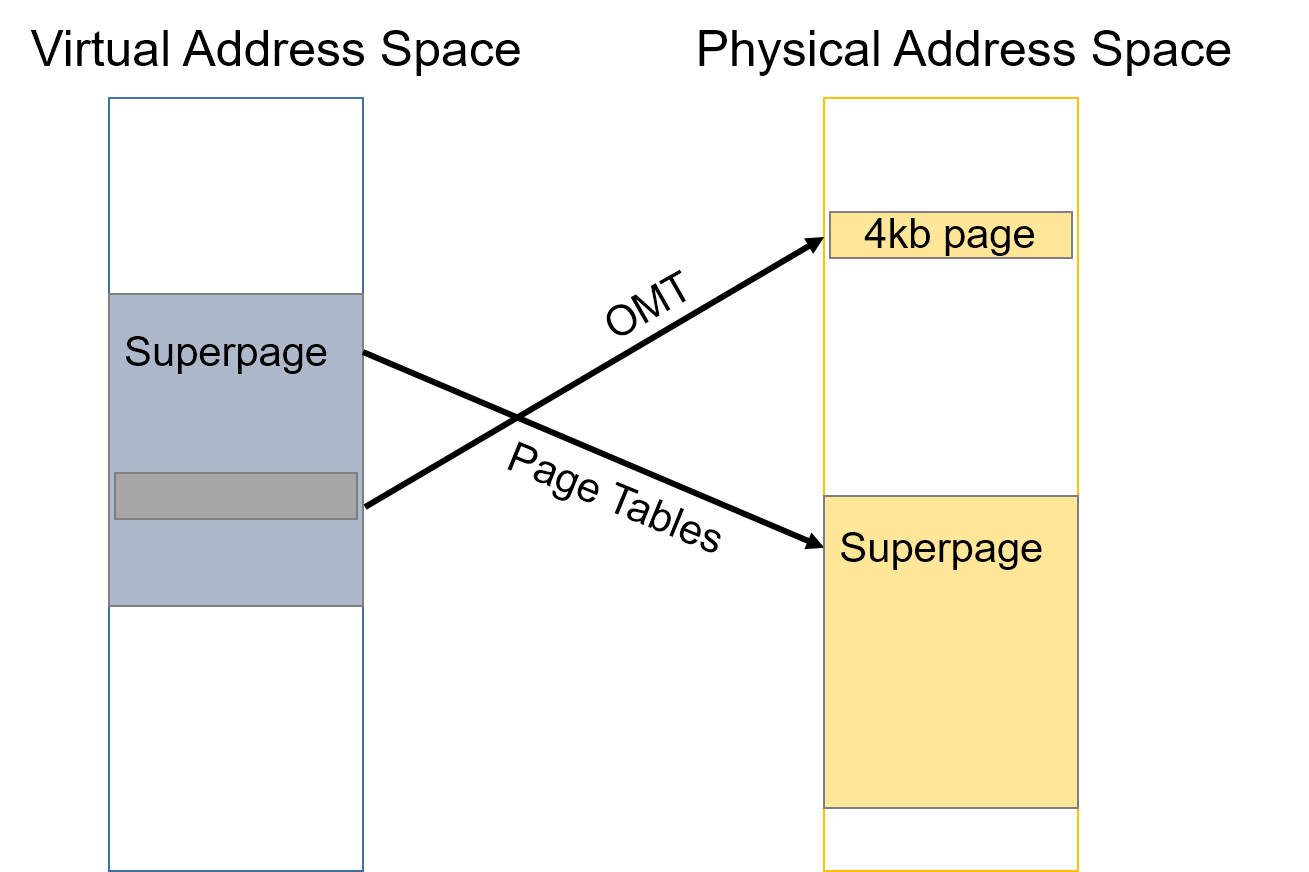
\includegraphics[width=3in]{Figures/Picture1}
    \caption{A basic diagram of the virtual-to-physical mappings for a superpage with overlay}
    \label{fig:basic}
\end{figure}
